\section{Resultados}

Todos los tiempos están en segundos y, cuando corresponde, se reporta la \textbf{mediana} de las 10 corridas.

\subsection{Perfilado de CPU: dónde se va el tiempo}

El reporte de GProf para el kernel secuencial es concluyente:

\begin{center}
\begin{tabular}{|l|r|r|r|}
\hline
\textbf{Función} & \textbf{\% tiempo propio} & \textbf{llamadas} & \textbf{ms/llamada} \\
\hline
\texttt{multiplicar\_y\_medir} & 100.13 & 1 & 140.19 \\
\texttt{llenar\_matrices\_con\_semilla} & 0.00 & 1 & 0.00 \\
\texttt{reservar\_matrices} & 0.00 & 1 & 0.00 \\
\hline
\end{tabular}
\end{center}

El 100\% del tiempo propio está en la función del kernel, y el llenado y la reserva de memoria son marginales. Esto confirma la decisión de cronometrar solo la multiplicación. El reporte de la máquina B es idéntico en este punto, así que la observación generaliza a hardware de otro fabricante.

\subsection{Perfilado de memoria: el comportamiento de la caché}

Esta es la medición más relevante del trabajo, porque cuantifica la hipótesis que el caso de estudio 1 dejó como intuición. La tabla~\ref{tab:cachegrind} muestra los contadores de Cachegrind para las tres variantes del kernel, con $N=500$, en la máquina A.

\begin{table}[ht]
\centering
\scriptsize
\begin{tabular}{|l|c|r|r|r|r|}
\hline
\textbf{Variante} & \textbf{T} & \textbf{I refs} & \textbf{D refs} & \textbf{D1 misses} & \textbf{D1 miss rate (lect.)} \\
\hline
Secuencial (naive)  & 1  & 1\,031\,897\,709 & 389\,051\,874 & 58\,050\,493 & \textbf{22.4\%} \\
Transpuesto          & 1  &   907\,904\,738 & 389\,301\,885 &  7\,893\,064 & \textbf{3.0\%}  \\
OpenMP               & 1  & 1\,034\,704\,330 & 389\,325\,981 & 59\,227\,926 & 22.8\% \\
OpenMP               & 8  & 1\,062\,467\,457 & 393\,297\,061 & 59\,226\,557 & 22.5\% \\
OpenMP               & 16 & 1\,034\,768\,697 & 389\,344\,956 & 59\,231\,589 & 22.8\% \\
\hline
\end{tabular}
\caption{Métricas de caché medidas con Cachegrind ($N=500$, máquina A). D1 miss rate corresponde a las lecturas de datos.}
\label{tab:cachegrind}
\end{table}

Tres observaciones se desprenden directamente:

\begin{enumerate}
    \item \textbf{La transposición de $B$ reduce los fallos de caché L1 en un factor 7.4}: de 58.05 millones a 7.89 millones, y la tasa de fallo de lectura baja de 22.4\% a 3.0\%. Es la medición experimental de la causa del buen rendimiento del kernel transpuesto.
    \item \textbf{El número de hilos no cambia la tasa de fallo}: OpenMP con $T=1$, $8$ y $16$ da 22.8\%, 22.5\% y 22.8\%. La tasa de fallo es una propiedad del \emph{patrón de acceso}, no del paralelismo: el kernel con OpenMP es el mismo kernel naive, con el mismo acceso a $B$ por columna.
    \item \textbf{La transposición además reduce las instrucciones ejecutadas} en un 12\% (de 1\,032 millones a 908 millones), porque el acceso contiguo a $B$ es más amigable con el planificador del compilador.
\end{enumerate}

\begin{figure}[ht]
\centering
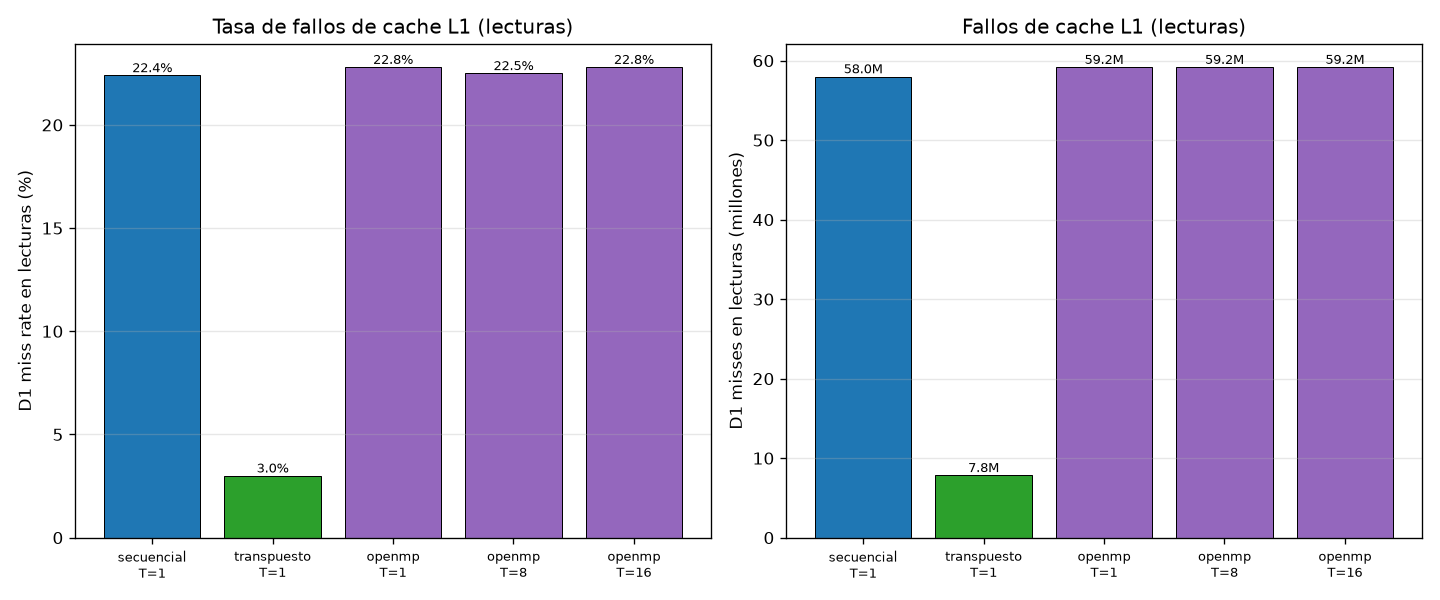
\includegraphics[width=0.95\textwidth]{figuras/cache_miss_rate.png}
\caption{Tasa de fallo de caché L1 en lecturas (izquierda) y cantidad absoluta de fallos (derecha) por variante del kernel. El transpuesto (verde) reduce la tasa de 22.4\% a 3.0\%.}
\label{fig:cache-miss}
\end{figure}

El \textbf{footprint de memoria} (max RSS) es prácticamente idéntico en todas las variantes: 4.3--4.7\,MB, que corresponde a las tres matrices de $N \times N$ enteros más el \emph{overhead} de las pilas de hilo. La memoria que consume el algoritmo depende solo del tamaño de las matrices, no del hardware ni del paralelismo.

\subsection{Desempeño: las cinco estrategias comparadas}

Para OpenMP se reporta el mejor $T$ por $N$, con la misma metodología que se aplicó a pthreads y a fork.

\begin{table}[ht]
\centering
\scriptsize
\setlength{\tabcolsep}{3pt}
\begin{tabular}{|c|r|r|r|r|r|r|r|r|r|r|r|}
\hline
\textbf{N} & \textbf{T\_seq} & \textbf{T\_pth} & \textbf{T\_fork} & \textbf{T\_full} & \textbf{T\_mem} & \textbf{T\_omp} & \textbf{s\_pth} & \textbf{s\_fork} & \textbf{s\_full} & \textbf{s\_mem} & \textbf{s\_omp} \\
\hline
500  & 0.0440 & 0.0315 (16) & 0.0152 (8) & 0.0459 & 0.0377 & 0.0160 (16) & 1.40 & 2.89 & 0.96 & 1.17 & \textbf{2.75} \\
1000 & 0.4230 & 0.2043 (16) & 0.1169 (16) & 0.4301 & 0.3019 & 0.1179 (16) & 2.07 & 3.62 & 0.98 & 1.40 & \textbf{3.59} \\
2000 & 4.3626 & 1.6430 (16) & 1.9805 (8) & 5.8909 & 2.6586 & 1.2786 (16) & 2.66 & 2.20 & 0.74 & 1.64 & \textbf{3.41} \\
4000 & 75.6511 & 24.2927 (16) & 59.1421 (8) & 70.0332 & 21.3223 & 16.6689 (8) & 3.11 & 1.28 & 1.08 & 3.55 & \textbf{4.54} \\
\hline
\end{tabular}
\caption{Tiempos (s, mediana de 10 corridas) y speedups de las cinco estrategias. La base es el secuencial con $-O2$. Entre paréntesis, el mejor $T$ de cada estrategia paralela.}
\label{tab:cinco-estrategias}
\end{table}

\begin{figure}[ht]
\centering
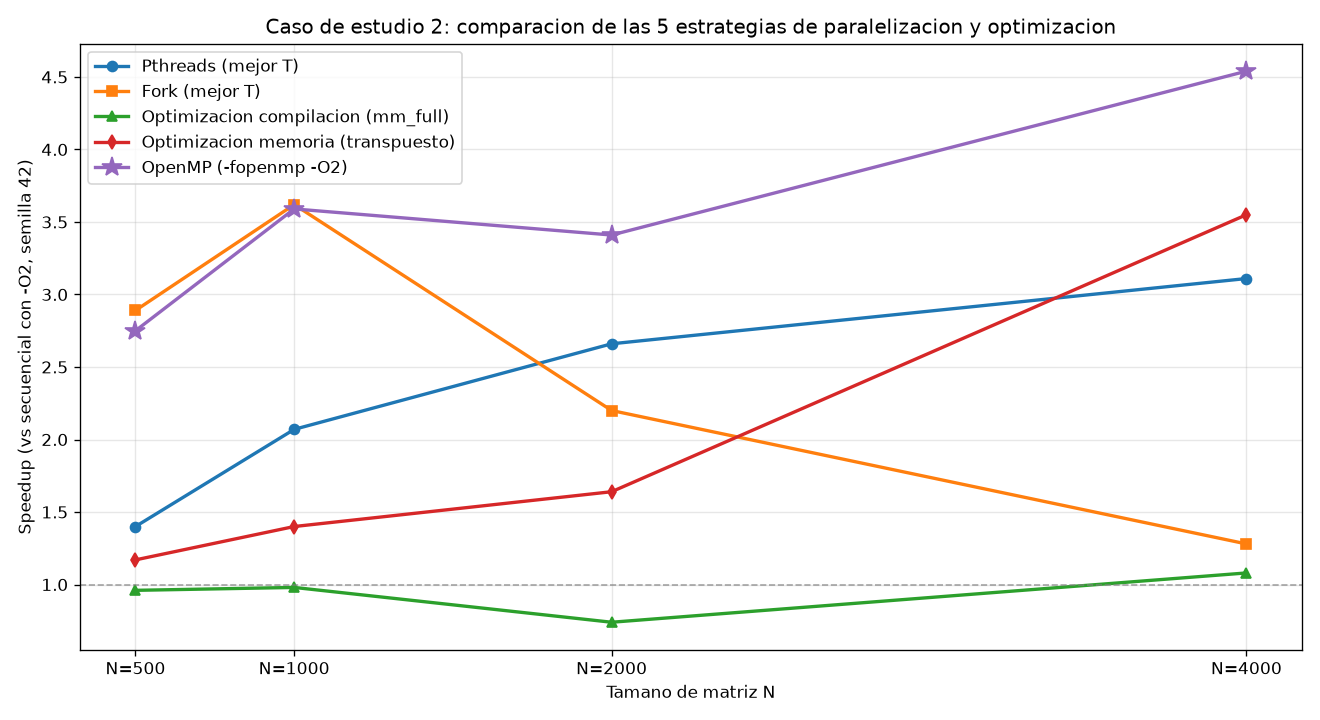
\includegraphics[width=0.9\textwidth]{figuras/comparativa_5_estrategias.png}
\caption{Speedup de las cinco estrategias frente al secuencial. OpenMP (estrella morada) es la estrategia más rápida en tres de los cuatro tamaños.}
\label{fig:5-est}
\end{figure}

\subsection{Escalamiento de OpenMP}

\begin{table}[ht]
\centering
\begin{tabular}{|c|r|r|r|r|r|c|}
\hline
\textbf{N} & \textbf{T=1} & \textbf{T=2} & \textbf{T=4} & \textbf{T=8} & \textbf{T=16} & \textbf{Speedup} \\
\hline
500  & 0.0450 & 0.0276 & 0.0239 & 0.0180 & \textbf{0.0160} & 2.81$\times$ \\
1000 & 0.4257 & 0.2385 & 0.1652 & 0.1473 & \textbf{0.1179} & 3.61$\times$ \\
2000 & 4.3026 & 2.7034 & 1.5880 & 1.4391 & \textbf{1.2786} & 3.36$\times$ \\
4000 & 76.0226 & 34.3422 & 18.0106 & \textbf{16.6689} & 18.0214 & 4.56$\times$ \\
\hline
\end{tabular}
\caption{Tiempos (s) de OpenMP por cantidad de hilos y speedup resultante respecto al $T=1$ de la misma máquina.}
\label{tab:escalamiento}
\end{table}

Con $T=16$ y $N=4000$ el tiempo \emph{empeora} frente a $T=8$ (18.02\,s contra 16.67\,s): la máquina tiene 12 núcleos lógicos, de modo que 16 hilos obligan al sistema a planificar más trabajo del que puede ejecutar en paralelo, y ese \emph{overhead} se come la ganancia.

\subsection{Benchmark entre las dos máquinas}

Las dos máquinas son hardware realmente distinto: distinto fabricante, distinta arquitectura, distinta jerarquía de caché y distinto sistema operativo.

\begin{table}[ht]
\centering
\small
\begin{tabular}{|l|l|l|}
\hline
\textbf{Característica} & \textbf{Máquina A} & \textbf{Máquina B} \\
\hline
CPU & Intel Core i5-12450HX (Alder Lake) & AMD Ryzen 5 5500U (Zen 2) \\
Núcleos físicos / lógicos & 8 / 12 & 6 / 12 \\
Caché L1d / L2 / L3 & 320 KiB / 7 MiB / 12 MiB & 192 KiB / 3 MiB / 8 MiB \\
Memoria RAM & 15 GiB & 11 GiB \\
Sistema operativo & Debian GNU/Linux 13 & Fedora Linux 41 \\
Compilador & gcc 14.2.0 & gcc 14.2.1 \\
\hline
\end{tabular}
\caption{Hardware de las dos máquinas del benchmark.}
\label{tab:hardware}
\end{table}

\begin{table}[ht]
\centering
\scriptsize
\setlength{\tabcolsep}{3.5pt}
\begin{tabular}{|c|r|r|r|r|r|c|r|r|c|}
\hline
\textbf{N} & \textbf{T\_A (s)} & \textbf{T\_B (s)} & \textbf{GOP/s A} & \textbf{GOP/s B} & \textbf{\%$\Delta$} & \textbf{Gana rend.} & \textbf{s\_A} & \textbf{s\_B} & \textbf{Gana sp.} \\
\hline
500  & 0.0160 (16) & 0.0215 (16) & 15.60 & 11.62 & $-25.5\%$ & \textbf{A} & 2.81$\times$ & 3.56$\times$ & \textbf{B} \\
1000 & 0.1179 (16) & 0.2291 (16) & 16.96 &  8.73 & $-48.5\%$ & \textbf{A} & 3.61$\times$ & 4.31$\times$ & \textbf{B} \\
2000 & 1.2786 (16) & 3.2704 (8)  & 12.51 &  4.89 & $-60.9\%$ & \textbf{A} & 3.36$\times$ & 3.20$\times$ & \textbf{A} \\
4000 & 16.6689 (8) & 59.9067 (8) &  7.68 &  2.14 & $-72.2\%$ & \textbf{A} & 4.56$\times$ & 3.53$\times$ & \textbf{A} \\
\hline
\end{tabular}
\caption{Benchmark entre las dos máquinas. Entre paréntesis, el mejor $T$ de hilos de cada equipo. ``\%$\Delta$'' es $(R_B-R_A)/R_A \times 100$ con $R=1/T$. ``Gana rend.'' identifica la más rápida y ``Gana sp.'' la que mejor paraleliza.}
\label{tab:benchmark-maquinas}
\end{table}

\begin{figure}[ht]
\centering
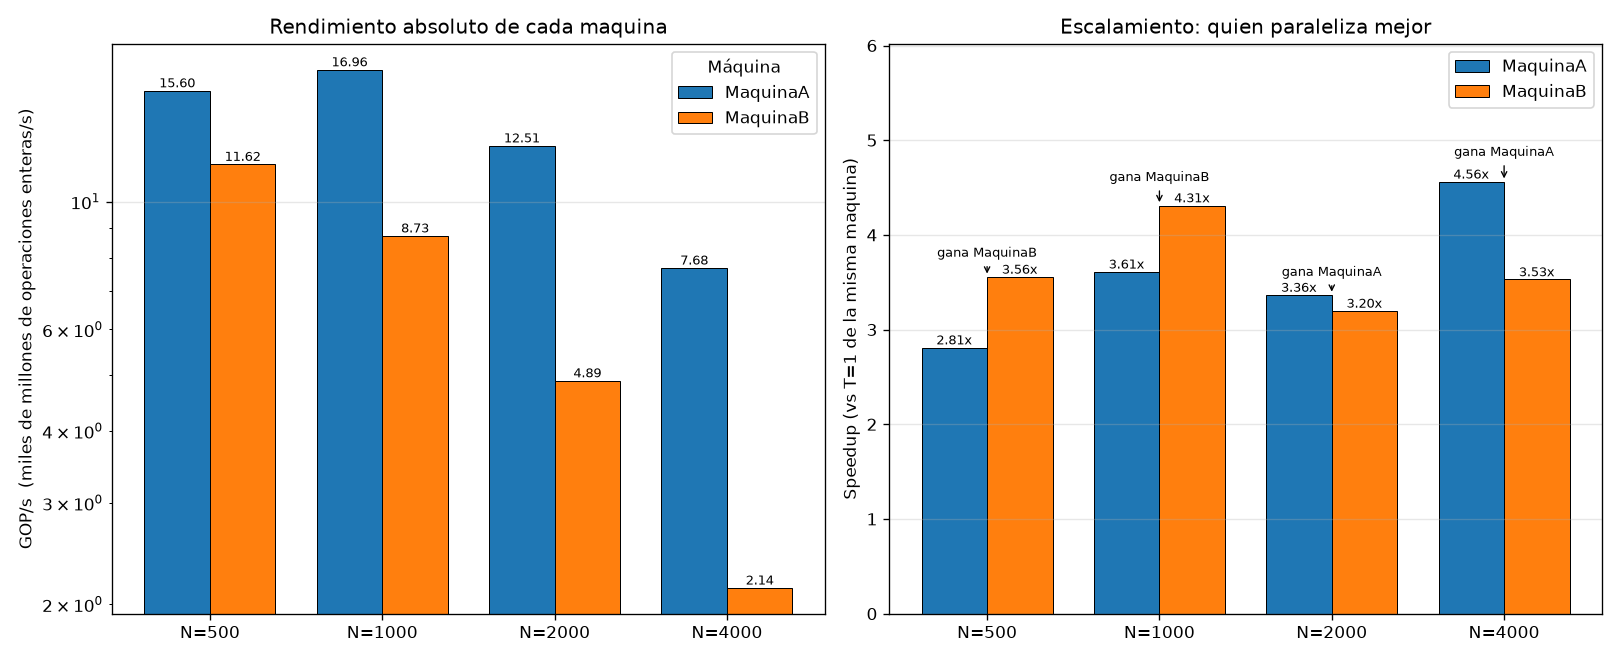
\includegraphics[width=0.98\textwidth]{figuras/benchmark_rendimiento.png}
\caption{Benchmark entre máquinas. Izquierda: rendimiento absoluto en GOP/s; la máquina A gana en todos los tamaños. Derecha: speedup interno con el ganador anotado; la B gana en $N=500$ y $N=1000$, la A en $N=2000$ y $N=4000$.}
\label{fig:benchmark-rendimiento}
\end{figure}
